\documentclass[12pt]{article}
\usepackage{cite}
\usepackage{fixltx2e}
\usepackage{graphicx}
\usepackage{float}
\usepackage{array}
\usepackage{longtable} 

\begin{document}
 

\section{Introduction}
 
This has been a long standing open problem to provide an interface on which a user, who has no idea about the syntax and working of a structured query language also known as SQL, can write queries in natural language and system converts that natural language to SQL. This SQL executes on database in order to fetch results. Many research has been done on this and still going on in order to bring up the accuracy. Although currently developed models are giving us a accuracy greater than 80\%, there are some dependencies in the model which makes them not suitable to use in practical applications. We will be discussing them as well.
\\ \\
 Relational databases store a vast amount of data and are accessed through structured query languages. Many non technical persons are not familiar with these structured query languages, which creates a lot of trouble and dependencies. If we can remove this structured query language (SQL) dependency, then it would be a lot easier to fetch data from databases. This problem has been given a lot of attention after great number of  large scale datasets has been made available \cite{zhong2017seq2sql} \cite{setlur2019inferencing} \cite{yu2018spider}. 
\\ \\
Pre trained language models such as BERT \cite{devlin2018bert} and RoBERTa \cite{liu2019roberta}  have gained a lot of success in the area of natural language processing tasks. \cite{guo2019content} has done some amazing work using BERT on WikiSQL dataset. It has utilized the pre-trained model BERT as well as database table content in order to achieve state of the art model with highest accuracy. This comes with some limitations which we will discuss in related work. 
\\Although there are number of models having significant accuracies on WikiSQL dataset, accuracies are still limited on Spider benchmark\cite{yu2018spider}. One of the reasons is that Spider dataset is more complex compared to WikiSQL dataset. WikiSQL focuses on rather simpler queries having single or multiple where clauses and no joins.\\
\\
We have used RoBERTa model to achieve our task. We used RoBERTa model
embeddings along with two knowledge vectors, namely, header knowledge
and question knowledge vectors and passed it to LSTM based models to give
us final results. We have improved both knowledge vectors which are passed
to LSTM based models. The proposed method in the study has been evaluated on WikiSQL dataet. We use 6 LSTM based models for predicting
individual parts of SQL. Significant improvements have been seen in each
of the sub models which adds up to total accruacy. Model responsible for
predicting select column has improved 1.0\%, select agg 0.2\%, where number
0.8\%, where column 2.7\%, where op 4.5\%, where value 5.4\%, which makes
our test execution accuracy increased by 5.5\%.
 


\newpage




\section{Research Methodology}
\subsection{Dataset}
WikiSQL is a large semantic parsing dataset. It contains around 24,241 tables and 80,654 natural language questions and it has corresponding structured query languages to those questions. Releasing this dataset has brought much attention to NLP2SQL task. Having this big dataset, it has enabled deep neural techniques to adopt this task. However, it contains simpler queries which do not have any joins and have at most one relation. 
\begin{figure}[H]
    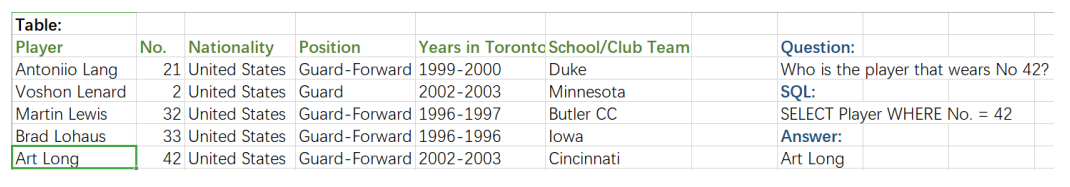
\includegraphics[width=450pt]{wikisql}
	\caption{An example of WikiSQL dataset}
    \label{fig:WikiSQL}
\end{figure}


\subsection{Implementation}
We have utilised RoBERTa, in order to build up our implementation on top of it. In the following section, we will be going through our implementation along with advantages and disadvantages. 

\subsection{RoBERTa}
In RoBERTa based model, we generate two knowledge vectors to give our model more confidence \cite{pal2021data}. These two are binary vectors and tell model which part are more important and need to be focused on by marking that specific parts. They encode the significance of headers and question tokens. Both of these vectors are then concatenated together and passed as additional features to model in order to bring more confidence in models. 


\subsubsection{Question Mark Vector}
\begin{figure}[H]
    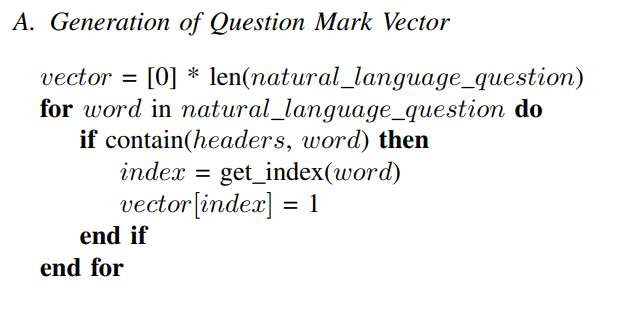
\includegraphics[width=300pt]{QMV}
    \caption{Question Mark Vector}
    \label{fig:Question mark vector}
\end{figure}

First, vector is initialized of same length as natural language question and assigned all the zeros in Fig 2. After initialization, program loops on natural language question tokens. Headers and each token of natural language question is passed in "contains" function which returns true if the token exists in headers, and false if it does not exist. If the token exists in header, then token index position is marked in vector with 1, otherwise, value remains 0 as per initialization. 


\subsubsection{Header Mark Vector}
\begin{figure}[H]
    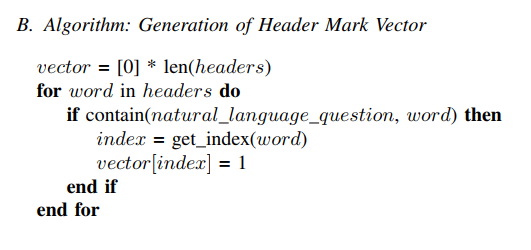
\includegraphics[width=300pt]{HMV}
    \caption{Header Mark Vector}
    \label{fig:Header mark vector}
\end{figure}

For header mark vector, we follow same procedure. Frist, vector is initialized of same length as headers and assigned all the values to zero in Fig 3. After initialization, program loops on headers. Each header and natural language question is passed in "contains" function which returns true if the header exists in questions, and false if it does not exist. If the header exists in question, then header index position is marked in vector with 1, otherwise, value remains 0 as per initialization. One thing to notice here is that loop iteration is not over headers here, rather it is on individual words in headers. Moreover, one thing that is majorly different here from \cite{guo2019content} is that we do not iterate through data here, hence maintaining the data integrity and privacy.
 

\subsection{Model}
Sequence to sequence style model is not recommended to use here because of the "order-matters" problem. It is possible for SQL query to have more than one correct queries. It is possible to move some conditions ordering and still get correct result. However, sequence to sequence style model choses one ordering correct and it labels other queries as wrong. In order to overcome this issue, another approach is used here suggested by SQLNet \cite{xu2017sqlnet}. It uses sketch based approach to predict SQL queries. However, unlike sequence to sequence, it eliminates the task of predicting complete queries and reduced that task into predicting some parts of it only. Hence the order matters problem is eliminated here. SQL query sketch:
 
\begin{figure}[H]
    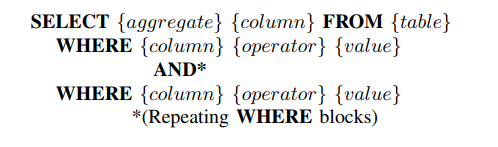
\includegraphics[width=300pt]{sketch}
    \caption{Query Sketch}
    \label{fig:Query Sketch}
\end{figure}

In fig 3, we can see all the parts which will be filled by models predictions instead of complete queries. 
\\
\\
Natural language question along with table headers is given input to RoBERTa model. It gives us embeddings which are then used for downstream tasks.  These embeddings along with the concatenation of question mark vector and header mark vector is passed into sub models in order to predict and fill SQL sketch. Model architecture is shown in Fig 5. 

\begin{figure}[H]
    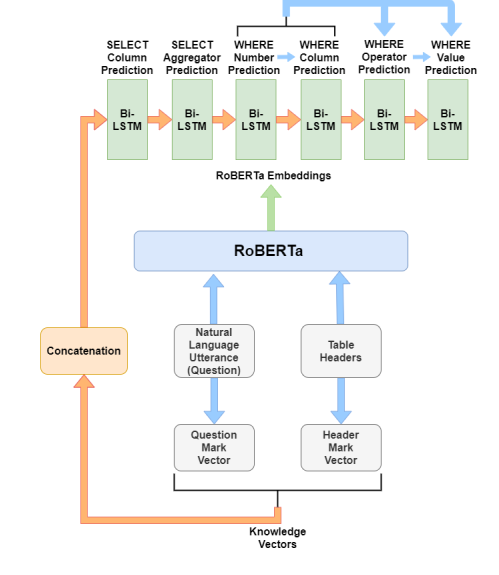
\includegraphics[width=350pt]{model}
    \caption{Model Architecture}
    \label{fig:Model Architecture}
\end{figure}

Embedding layer in this architecture plays an important role. Since we pass two knowledge vectors as well along with RoBERTa embedding into sub models for downstream tasks, it is important to not make our model depend on these two knowledge vectors completely. It is because there is a possibility that natural language question does not match with headers token, hence, not giving much information. If there are no matches between natural language questions and header tokens, then vectors would be consisting of zeros and would not give much information to model. Therefore, embeddings is very important and that is why RoBERTa embeddings is used here. 
\\
\\
It is important for model to extract significance amount of information from natural language question and table headers. Hence, both of these information is passed in RoBERTa model as shown in Fig 4. Similar architecture is used in \cite{guo2019content}, but vectors are generated using table content, hence, compromising data privacy. Another reason to use RoBERTa model is to have some sense of knowledge and context in model so that it can understand the meaning is same of even mismatched tokens. RoBERTa is pre trained on very large corpus of 160 GB and on masked language modeling, next sentence predictions tasks. This gives the model desired sense of knowledge and context. 


 
\subsection{Enrichment via Similar Sense Words}
We have built our experiment on top of the RoBERTa model. 

\subsubsection{Similar Sense Words}
The WordNet database contains many sorts of relationships between words which help us understand relations between different words. It can categorize words into different hierarchies and answer many interesting questions. If we have a single word "run" and we would like to understand its sense and relations between different words which are in close proximity to it. WordNet helps us understand different senses and different relations of words with each other. Example shown in figure \ref{wordnet}.


\begin{figure}[H]
    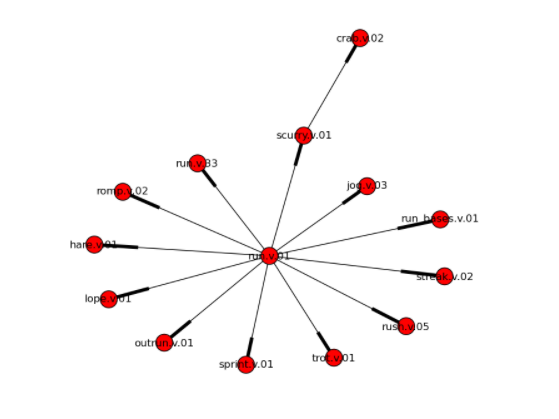
\includegraphics[width=400pt]{wordnet}
    \caption{WordNet}
    \label{wordnet}
\end{figure}

\subsubsection{Implementation}
We have taken help of WordNet in creating of our two knowledge vectors, header knowledge vector and question knowledge vector. While marking these vectors in order to provide useful information to model with the areas where to focus on, we used to look for exact matches in the headers and questions. Through this method, our vectors were loosing much information which could help model gain some accuracy and show better results. In our implementation, we did not look for exact matches, rather, we created two synsets and calculated the probability of their match which helped us better understand the relations of words rather than comparing it straightforward. We marked vectors if the probability was greater than or equal to 0.7. 

\subsubsection{why?}
It is quite common in natural language that we sometimes use synonyms in our sentences and not exact words which were affecting results in our problem domain. Not only synonyms, but the use of singular words and plural words were also affecting our model, since, singular and plural does not result in exact match as well. 

\subsubsection{Analysis}
When we started enriching the header and knowledge vectors with the help of similar sense words, we started tracking how many words were benefiting from it. We started tracking count of words which were completely same and count of those words as well which were close to each other. This gives us the clear picture in terms of percentage that how many words are being benefitted from our implementation. Comparison can be seen in figure \ref{WordMatches}.

\begin{figure}[H]
    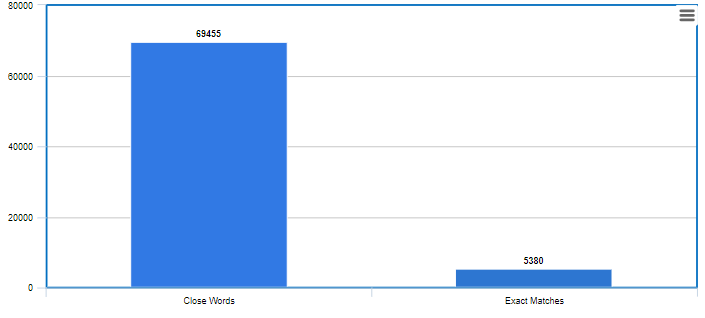
\includegraphics[width=450pt]{wordmatches}
	\caption{Word Matches}
    \label{WordMatches}
\end{figure}

\section{Findings}


We have evaluated our model on the WikiSQL dataset with
the logical form and execution accuracy metrics. The method
of calculating the execution accuracy does involve the model
querying the database which goes against our core objective of
data privacy, but this is not a necessary step and neither does
it affect the model’s training in any way. The only purpose of
such querying is to obtain an additional evaluation metric to
better understand our model’s performance. The final model
when deployed would not need to calculate any such metrics,
thus keeping the data completely private.
We have compared our model with the state of the art model
as well as the baseline SQLNet Model:
Note: Accuracy has been shortened to acc. and execution
has been shortened to exec.

 


\subsection{RoBERTa with Traditional Knowledge Vectors}

We implemented RoBERTa model without using table data. It did ensure the privacy of data, however, it did come with its trade off. We marked two knowledge vectors using only headers and natural language question. In this model, we did not use any real data for training of the model, rather, we used only schema information of the table. Results are shown in table \ref{robertatable} and table \ref{robertatabledetailed}.

 \begin{table}
\centering
 \begin{tabular}{| m{2cm} | m{2cm}| m{2cm} |m{2cm}| m{2cm} |} 
 \hline
Model & Dev logical form acc. & Dev exec acc. & Test logical form acc. & Test exec acc. \\ 
 \hline\hline
  RoBERTa & 74.4\% & 80.9\% & 73.3\% & 80.3\% \\ 
 \hline
\end{tabular}
\caption{Overall result of RoBERTa Model on WikiSQL task}
\label{robertatable}
\end{table}


\begin{table}
\centering
 \begin{tabular}{| m{2cm} | m{2cm}| m{2cm} |m{2cm}| m{2cm} |m{2cm} | m{2cm} |m{2cm} |} 
 \hline
  Dataset & SELECT column & SELECT agg & WHERE number & WHERE column & WHERE op & WHERE value\\ 
 \hline\hline
  Dev & 96.2\% & 90.6\% & 98.0\% & 91.3\% & 93.4\% &  90.5\% \\ 
\hline
 Test & 95.8\% & 90.4\% & 97.2\% & 89.8\% & 92.4\% &  89.7\% \\ 
 \hline

\end{tabular}
\caption{Break down result of RoBERTa model on WikiSQL task}
\label{robertatabledetailed}
\end{table}

\subsection{RoBERTa Model with Header Knowledge Vector with WordNet}

We implemented RoBERTa model without using table data. We marked two knowledge vectors using only headers and natural language question. However, the main difference here is how we did the  encoding of Header knowledge vector. We encoded vector here with the help of WordNet as explained in Section 6. Results are shown in table \ref{robertatableoneheader} and table \ref{robertatabledetailedoneheader}.



 \begin{table}
\centering
 \begin{tabular}{| m{2cm} | m{2cm}| m{2cm} |m{2cm}| m{2cm} |} 
 \hline
Model & Dev logical form acc. & Dev exec acc. & Test logical form acc. & Test exec acc. \\ 
 \hline\hline
  RoBERTa & 81.0\% & 86.0\% & 80.4\% & 85.4\% \\ 
 \hline
\end{tabular}
\caption{Overall result of RoBERTa Model on WikiSQL task with WordNet Header vector}
\label{robertatableoneheader}
\end{table}


\begin{table}
\centering
 \begin{tabular}{| m{2cm} | m{2cm}| m{2cm} |m{2cm}| m{2cm} |m{2cm} | m{2cm} |m{2cm} |} 
 \hline
  Dataset & SELECT column & SELECT agg & WHERE number & WHERE column & WHERE op & WHERE value\\ 
 \hline\hline
  Dev & 97.0\% & 90.8\% & 98.8\% & 93.8\% & 97.7\% &  95.6\% \\ 
\hline
 Test & 96.8\% & 90.6\% & 98.3\% & 93.3\% & 97.2\% &  95.2\% \\ 
 \hline

\end{tabular}
\caption{Break down result of RoBERTa model on WikiSQL task with WordNet Header vector}
\label{robertatabledetailedoneheader}
\end{table}


\subsection{RoBERTa Model with Question \& Header Knowledge Vectors with WordNet}

We implemented RoBERTa model without using table data. We marked two knowledge vectors using only headers and natural language question. However, the main difference here is how we did the  encoding of Header knowledge vector as well as Question knowledge vector. We encoded vectors here with the help of WordNet as explained in Section 6. Results are shown in table \ref{robertatabletwoheader} and table \ref{robertatabledetailedtwoheader}.

 \begin{table}
\centering
 \begin{tabular}{| m{2cm} | m{2cm}| m{2cm} |m{2cm}| m{2cm} |} 
 \hline
Model & Dev logical form acc. & Dev exec acc. & Test logical form acc. & Test exec acc. \\ 
 \hline\hline
  RoBERTa & 81.4\% & 86.6\% & 80.5\% & 85.8\% \\ 
 \hline
\end{tabular}
\caption{Overall result of RoBERTa Model on WikiSQL task with WordNet Header \& Question vectors}
\label{robertatabletwoheader}
\end{table}


\begin{table}
\centering
 \begin{tabular}{| m{2cm} | m{2cm}| m{2cm} |m{2cm}| m{2cm} |m{2cm} | m{2cm} |m{2cm} |} 
 \hline
  Dataset & SELECT column & SELECT agg & WHERE number & WHERE column & WHERE op & WHERE value\\ 
 \hline\hline
  Dev & 97.2\% & 90.8\% & 98.8\% & 94.0\% & 97.9\% &  95.9\% \\ 
\hline
 Test & 96.7\% & 90.7\% & 98.3\% & 93.4\% & 97.3\% &  95.3\% \\ 
 \hline

\end{tabular}
\caption{Break down result of RoBERTa model on WikiSQL task with WordNet knowledge vectors}
\label{robertatabledetailedtwoheader}
\end{table}

\subsection{Comparison of Final Results}
Final comparison of test results are shown in table \ref{finalcomparisonmodel} and table \ref{finalcomparison}.


 \begin{table}
\centering
 \begin{tabular}{| m{2cm} | m{2cm}| m{2cm} |m{2cm}| m{2cm} |} 
 \hline
Model & Dev logical form acc. & Dev exec acc. & Test logical form acc. & Test exec acc. \\ 
 \hline\hline
   RoBERTa base Model & 74.4\% & 80.9\% & 73.3\% & 80.3\% \\ 
  Our Model & 81.4\% & 86.6\% & 80.5\% & 85.8\% \\ 
 \hline
\end{tabular}
\caption{Comparisons of base and our final Model.}
\label{finalcomparisonmodel}
\end{table}


\begin{table}
\centering
 \begin{tabular}{| m{2cm} | m{2cm}| m{2cm} |m{2cm}| m{2cm} |m{2cm} | m{2cm} |m{2cm} |} 
 \hline
  Model & SELECT column & SELECT agg & WHERE number & WHERE column & WHERE op & WHERE value\\ 
 \hline\hline
  RoBERTa base model & 95.8\% & 90.4\% & 97.2\% & 89.8\% & 92.4\% &  89.7\% \\ 
\hline
 Our Model &  96.7\% & 90.7\% & 98.3\% & 93.4\% & 97.3\% &  95.3\% \\ 
 \hline
\end{tabular}
\caption{Comparisons of base and our final sub Models.}
\label{finalcomparison}
\end{table}


\section{Conclusion}
In this experiment, the focus was on improving the model without using the data available in database due to obvious privacy issues. This is a data agnostic model. We have seen that existing models use table content as well as a feature when inputting the model. Moreover, if some models are not using the real data, they make use of execution guided decoding. We have not used any of these two techniques. We have developed a data blind model using only table schema and two important knowledge vectors with the help of WordNet. 
\\
\\
Our results show promising improvements when even one vector is implemented with WordNet. Moreover, slightly more improvement is seen when both knowledge vectors where marked with the help of WordNet. Comparison between one vector, both vectors and no vectors for dev dataset is shown in figure \ref{devset} and for test dataset is shown in figure \ref{testset}


\section{Future Work}
Our work opens a new direction to explore which can yield many promising results. There are many possibilities inside the work of finding a similar sense of words and enriching the knowledge vectors which can provide new insights of data to model. Moreover, there could be dynamically selection of probability values while finding the different senses among words. These new findings can be tried with our previous existing knowledge in different combinations which can lead to new dimensions of research. 



\begin{figure}[H]
    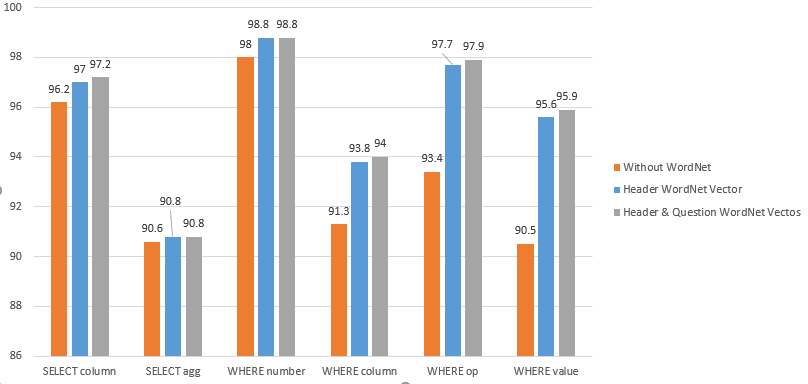
\includegraphics[width=400pt]{devset}
    \caption{Comparison betwen Without WordNet, Header WordNet \&  Question WordNet Vectors for Dev}
    \label{devset}
\end{figure}


\begin{figure}[H]
    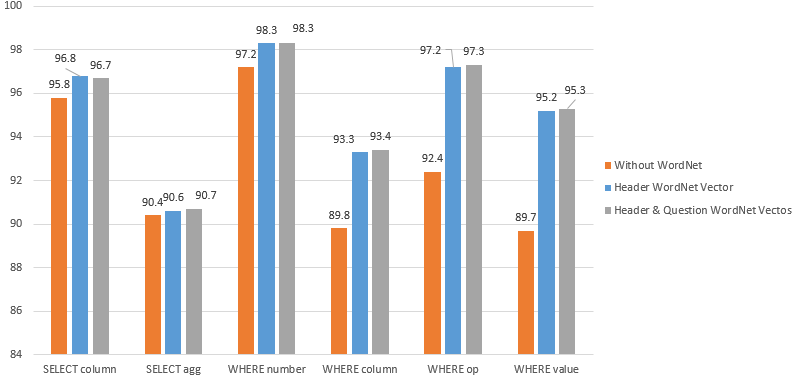
\includegraphics[width=400pt]{testset}
    \caption{Comparison betwen Without WordNet, Header WordNet \&  Question WordNet Vectors for Test}
    \label{testset}
\end{figure}

\bibliography{references}
\bibliographystyle{ieeetr}
\end{document}